\documentclass[12pt,journal,compsoc]{IEEEconf}
%\usepackage[english]{babel}
\usepackage[utf8]{inputenc}
\usepackage[T1]{fontenc}
\usepackage{graphicx}
\usepackage{amsmath,amssymb, mathtools, bm, gauss}
\usepackage{algorithm,algorithmic}
\usepackage{listings}
\usepackage{xcolor}
\usepackage{hyperref}
\usepackage{spverbatim}
\usepackage[]{pgfplots}
\usepackage{lscape}
\usepackage{lmodern}
\usepackage[labeled]{multibib}
%\usepackage[colorlinks=true]{hyperref}
\usepackage{varioref}

\renewcommand*\ttdefault{txtt}

\newcommand{\todo}[1]{{\color[rgb]{.5,0,0}\textbf{$\blacktriangleright$#1$\blacktriangleleft$}}}

\lstset{basicstyle=\footnotesize\ttfamily,breaklines=true}
\lstset{framextopmargin=50pt}

\pagestyle{plain}
\pagenumbering{arabic}

\begin{document}
\title{
\huge{I/O Algorithms}
\vskip0.5em
\large{I/O-efficient merge-sort 2014 - group 6}
}
\author{
Frederik Lønstrup Hansen\\ 20096365\\
	\and
Randi Katrine Hillerøe \\ 20103073 \\ 
	\and
Andreas Fyrstelin Kristiansen\\ 20092027 \\
	\and
Rasmus Kampmann Olsen\\ 20093692\\
}

\maketitle
\begin{abstract}
ANSVAR: ... rasmus? Har vi brug for et abstract? Der er jo som sådan intet nyt i det her, så tænker en introduction er nok
\end{abstract}

% see http://imf.au.dk/system/latex/bog/

\section{Introduction}

In this report we describe our implementation, experiments and results we have achieved during project 1 for I/O algorithms 2014.
As reading and writing to and from the disk is estimated at ${10^{6}}$ times slower than using RAM or the CPU cache, creating efficient I/O algorithms can mean the difference between getting a result within a reasonable time-frame and not. 
The usual memory model is made with a very small fast and local memory near CPU, a larger RAM, and finally the disk. Each level that is further away from the CPU becomes slower by a large factor. In our experiments and calculations we are only interested in calculating and experimenting with the time of the I/O operations. An I/O operation is defined by either a read from the disk to main memory or write from the main memory to the disk.



\section{Merge sort with streams}
This section describes our implementation of the 4 different required streams. 

\subsection{Single item stream}
The single item streams are the most simple implementation with no optimizations.

The input stream uses the C function \texttt{open} to open a file in read-only mode and the \texttt{read} function to read a single element from the file. To implement the \texttt{endOfStream} functionality we have actually implemented a single item buffer. The buffer is initially populated right after calling \texttt{open} and then updated every time \texttt{readNext} is called. This is done to know whether we have reached the end of the file or not. If no more can be read from the file when the buffer is updated we have reached the end.

The output stream opens a file in write-only mode. If the file does not exist it will be created. If the file does exist the file is truncated to ensure we write to an empty file.

\subsection{Fread and FWrite}
Fread and FWrite 


\subsection{Buffered}
Buffered input and output


\subsection{mmap/munmap}
mmap/munmap 

\section{D-way merge sort}

Our d-way merge sort takes d sorted input streams \textit{ins}, and creates an output stream with the elements from each stream in a sorted order. Merging takes place in the method \textit{merge}. We use a small helper class, streamHeader, where we can easily access the next element in the stream and start loading in the next element(s) if required. In this class there is a boolean flag called \textit{done}, which is used to check if an input stream should be included in the rebuilding of the heap after extracting an element from the streamHeader.
We use the standard c++ \textit{make_heap} function.

ANSVAR: rasmus...andreas?
D-way merge sort



\section{External Merge-sort}

results: Andreas? 

External merge sort



\section{Experiments}

All of our experiments are run with a limitation of 1mb RAM - a limitation we achieved by using cgroups in linux - on a standard mechanical hard-drive. This was done to significantly reduce the running time of our experiments and the amount of data required. 
During the first part of our testing we did in no way manage to get the expected results. In fact they were more or less opposite of the what the theory predicted. For example running the external merge sort with one small and one large N showed the larger N to be faster! We have not managed to find an adequate explanation for this so far and it would require require more investigation to find the reason.
We have however found a solution to the above problem, which gives results that fit the theory a lot better. By including an optimization flag for our compiler (in our case we used clang) not only did the running time decrease by roughly 1/3 but the results of the test cases also align better with the expected result. 

\subsection{Stream implementations}
The tests for our streams include testing different values of the buffersize b, the amount of streams d, and with a varying number of elements n. 
Each test has been run 100 times where the average is the values used in the graphs. 

\subsubsection{SingleItemStream and FStream}
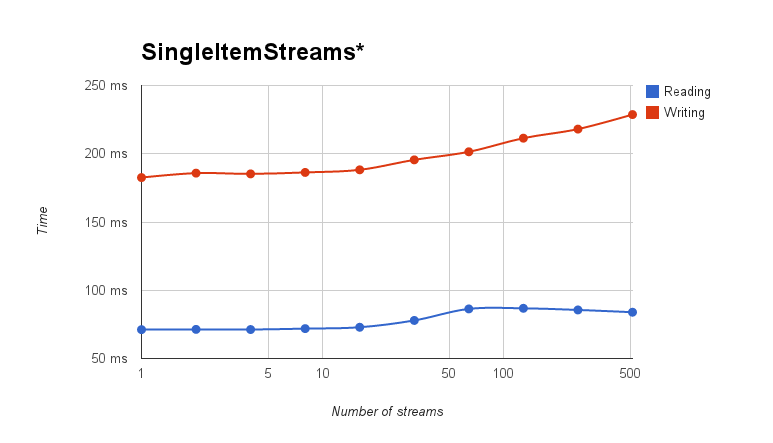
\includegraphics[width=90mm]{parts/SIS.png}
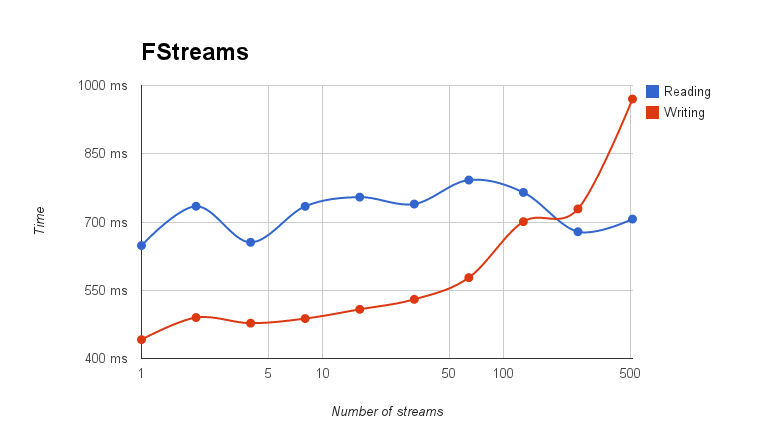
\includegraphics[width=90mm]{parts/FS.png}

The implementation of these streams does not require a manually set buffer size, this is because the OS or the compiler does this in advance. 

The SingleItemStream is behaving as expected; the number of streams does not affect reading very much, and writing increases a bit per stream added, but nothing significant, so it may be attributed to implementation flaws. 

The FStreams graph shows a wide variance in reading, but i stays within a 200ms range not dependant on the amount of streams. Writing on the other hand shows a rapid increase in performance after exceeding 64 streams. 

\subsubsection{BufferedStreams and MMappedStreams}
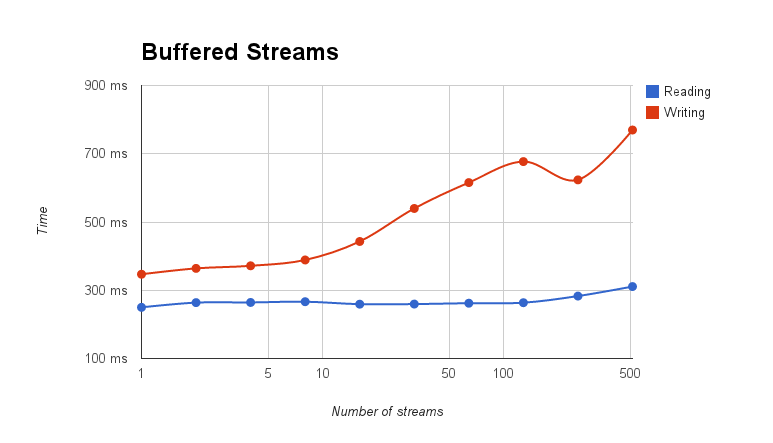
\includegraphics[width=90mm]{parts/BS.png}
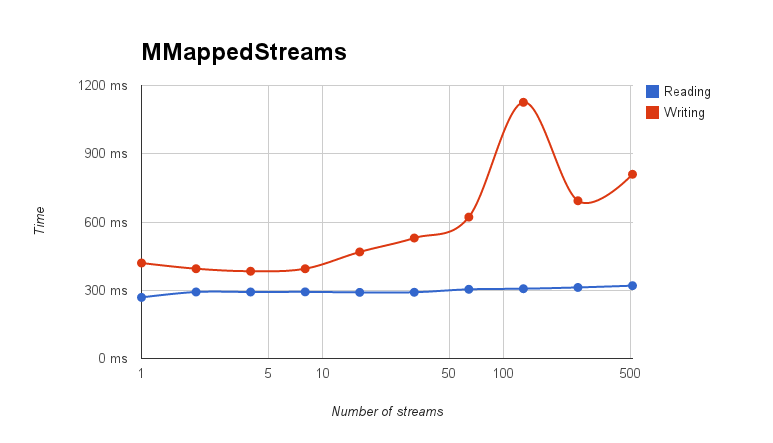
\includegraphics[width=90mm]{parts/MMS.png}
These tests was done with a buffer size of 1024, because this was shown to be the best one when we tested them based on buffersize. 

The BufferedStreams implementation does reading reasonably well, with no significant increase in performance, the writing on the other hand does worse with more streams, with a slight drop around 256 streams, just to continue its performance decline. 

The MMappedStreams behaves similarly to the BufferedStreams, except that the running time is just slightly worse. The running time is practically unchanged for reading, while writing increases in running time the more streams we add. The interesting thing to note here though, is the large decline in performance with a buffer size of 124, afterwards it drops again to expectable levels, and continues as such. 

\subsubsection{Comparing the streams}
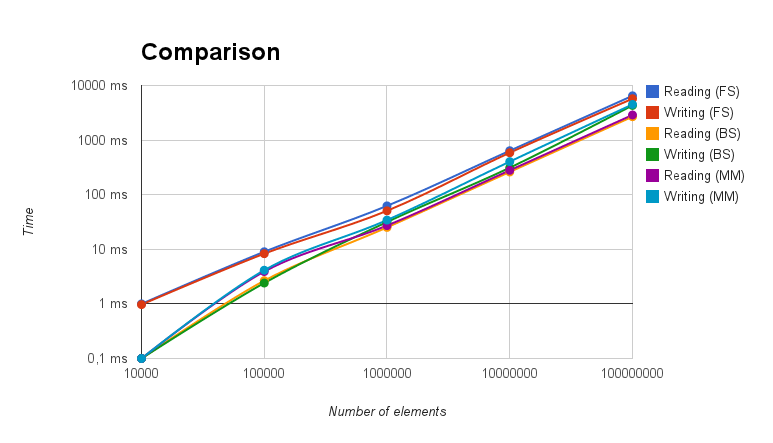
\includegraphics[width=90mm]{parts/StreamCompare.png}
Our comparison graph for the stream implmentaions contain only three of the streams. The single item stream was so slow with large amounts of elements that we did not finish the tests for that implementation. The other streams are closer performance-wise as the graph shows. The streams based on \texttt{fread} and \texttt{fwrite} are clearly slowest which match up with what we expected. Our own buffered implementation slightly outperforms the \texttt{mmap} implementation which is why we ended up chosing that as the streams for our merge sort algorithm.

\subsection{ Finding merge sort parameters}
Andreas


\section{External versus heap and quicksort}

Using the results from previous tests we declared a winning strategy for external sorting - bufferedStream with a buffer size of 1024k, a $d$ value of 32 and a $m$ of size 64k. We then ran this setup for several values of N. The same N values were used for a standard quicksort and heapsort implementation.

Heapsort's time grew extremely fast as soon as swap space had to be used for large values of N so eventually we decided to stop these tests as they would simply require to much time to complete. Heapsort is often hailed as having a worst case that is better than Quicksort, however this only happens for internal sorting as the required I/Os to maintain the heap far outweigh other time constrains.

Next we looked at Quicksort compared to external merge sort. We expected Quicksort to perform a lot better than Heapsort, and it did, however we had also expected the difference between quicksort and the external sort to be more in favour of external sorting as N gew. As can be see from the graph this was not always the case.

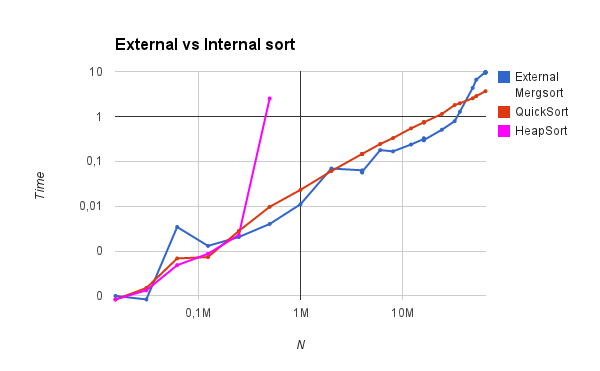
\includegraphics[width=90mm]{graphics/compare.png}

When the number of items to be sorted is low enough to fit into memory both heapsort and quicksort performs better than External - remember our memory is limited to 1 mb during this experiments - however as soon as that value is exceed external sorting becomes a lot better than Heapsorting. Quicksort on the other hand increases in a logarithm fashion seemingly no matter how large N became. In fact quicksort becomes faster than the external merge sort for very large vaules - this was not as we had predicated! More tests would be required to find the exact reason for this, but we suspect it is in fact due to implementation details of our merge sorting. We use Vectors to keep track of the paths and streams which may end up giving us a unnecessary large overhead. Up untill this point our merge sorting does out perform Quicksort.

\section{Conclusion}
Ansvar: Os alle !?

Oh wow I/O is slow shit!! You better make sure you do it in a smart way!




\pagebreak

\end{document}
